%%%%%%%%%%%%%%%%%%%%%%%%%%%%%%%%%%%%%%%%%%%%%%%%%%%%%%%%%%%%%%%%%
% Dissertacao de Mestrado / Dept Fisica, CFM, UFSC              %
% Andre@UFSC - 2011                                             %
%%%%%%%%%%%%%%%%%%%%%%%%%%%%%%%%%%%%%%%%%%%%%%%%%%%%%%%%%%%%%%%%%

%:::::::::::::::::::::::::::::::::::::::::::::::::::::::::::::::%
%                                                               %
%                          Capítulo 1                           %
%                                                               %
%:::::::::::::::::::::::::::::::::::::::::::::::::::::::::::::::%

%***************************************************************%
%                                                               %
%                         Introdução                            %
%                                                               %
%***************************************************************%

\chapter{Introdução}
\label{sec:Intro}

%***************************************************************%
%                                                               %
%                     Introdução - Nova era                     %
%                                                               %
%***************************************************************%

\section{A nova era da astronomia}
\label{sec:Intro:NovaEra}

Os primeiros levantamentos de dados da astronomia extragalática começaram a ser
feitos na década de 80 \citep{Huchra1988, Jones2005}. Foram observadas cerca de
2400 galáxias pelo {\em Center for Atrophysics} em Harvard \citep{Huchra1983} e
aproximadamente 2000 galáxias pelo {\em Southern Redshift Survey}
\citep{DaCosta1988}.

Com o advento dos {\em mega-surveys}\fixme, está começando uma revolução na
forma de fazer ciência na astronomia. Os diversos {\em surveys}\footnote{Um {\em
survey} astronômico é um levantamento ou mapeamento de regiões do céu utlizando
telescópios.} em execução atualmente estão produzindo dados a uma taxa da ordem
de petabytes por ano. Este talvez seja o primeiro campo da ciência onde as
informações coletadas por máquinas tenham -- nas próximas décadas -- um volume
maior do que os seres humanos são capazes de digerir. Uma espécie de {\em
Singularidade Tecnológica}\footnote{O termo {\em Singularidade tecnológica} se
refere a um futuro hipotético onde uma inteligência superior à humana emerge
através da tecnologia. Qualquer previsão após tal fato se torna muito difícil,
algo similar a um horizonte de eventos, dada a dificuldade em entender uma
inteligência superior à humana.} da astrofísica, onde máquinas coletam, analizam
e classificam dados. O papel do cientista num cenário como este ainda não está
muito claro \citep{Norris2010}.

\subsection{Mega-levantamentos de dados}

O {\em Sloan Digital Sky Survey} \citep[\SDSS]{York2000}, é referência quando
falamos em {\em surveys} modernos. Em seus 8\fixme anos de funcionamento, obteve
imagens em 5 filtros (ver figura \ref{fig:GalexFilters}) de um quarto do céu e
espectros de um milhão de galáxias. O seu catálogo contém 4 terabytes de dados
fotométricos e espectroscópicos, sem contar as imagens. O \SDSS foi praticamente
o primeiro {\em survey} a conseguir popularizar o acesso aos seus dados. Estes
foram feitos públicos desde o início\citneed, iniciando uma ``corrida do ouro''
no seu vasto volume de dados. Esta filosofia é compartilhada hoje pela grande
maioria dos {\em surveys} de grande porte.

Existem diversos {\em surveys} em operação atualmente. O {\em Wide-field
Infrared Survey Explorer} (WISE) é um telescópio espacial da NASA\footnote{{\em
NASA Explorer Mission} - \url{http://explorers.gsfc.nasa.gov/missions.html}},
que está mapeando o céu inteiro nas faixas de $3,4\mu$m, $4,6\mu$m, $12\mu$m e
$22\mu$m do infravermelho \citep{Wright2010}. O {\em Visible and Infrared Survey
Telescope for Astronomy} (VISTA) é um telescópio no Chile fazendo um {\em
survey} do céu do hemisfério sul no infravermelho próximo \citep{Born2010}.
Tratado com mais detalhes no capítulo \ref{sec:Galex}, o {\em Galaxy Evolution
Explorer} (\galex) mapeou o céu em ultravioleta. O {\em Kepler} é um telescópio
espacial da NASA \citep{Borucki2010}, semelhante ao WISE, e está fazendo um
survey de uma região da Via Láctea para descobrir a fração de estrelas com
planetas similares à Terra na nossa Galáxia. Convém mencionar também o {\em 2dF
Galaxy Redshift Survey} (2dFGRS) \citep{Colless1999} e o {\em Two Micron All Sky
Survey} (2MASS) \citep{Skrutskie2006}. Embora estes {\em surveys} já tenham sido
concluídos, os seus dados permanecem disponíveis publicamente.

O projeto JPAS ({\em Javalambre Physics of the Accelerating Universe Survey}) é
um {\em survey} que pretende mapear $8\,000$ graus quadrados do céu em 56
cores\citep{Benitez2009}. Os filtros, de banda estreita, irão cobrir toda a
região óptica, formando um espectro de baixa resolução para cada pixel do
survey. Serão mais de 200 terabytes de dados brutos\citneed. O projeto é uma
colaboração entre Espanha e Brasil, com mais de 70 pesquisadores e engenheiros
envolvidos. Integrantes do Grupo de Astrofísica da UFSC estão envolvidos neste
projeto\citneed. O objetivo do {\em survey} é a exploração das causas da
aceleração do universo, relacionadas à energia escura. Entretanto, uma
quantidade considerável de ciência adicional poderá ser feita com base no
espectro de uma região tão ampla do céu. Seu início está previsto para 2013.

O LSST ({\em Large Synoptic Survey Telecope}) mapeará metade do céu a cada mês,
aproximadamente, durante cerca de dez anos \citep{Ivezic2008}. As suas operações
científicas tem início previsto para 2020. Serão mais de um petabyte em imagens
brutas por ano, muito mais do que poderia ser revisado por humanos. Este {\em
survey} também pretende explorar a natureza da energia escura, embora, da mesma
forma que o JPAS, os dados possam ser aproveitados para diversos outros fins.

\subsection{Mineração de dados}

Tradicionalmente astrônomos armazenam seus dados em arquivos texto ou binários
contendo um registro por linha, de um forma tecnicamente conhecida como {\em
flat file}. Buscas neste tipo de banco de dados são feitas examinando
individualmente cada registro do arquivo. Com o volume de dados obtido pelo
\galex (aproximadamente 222 milhões de objetos, 34 mil campos), o uso de
arquivos simples para armazenamento de dados se torna inviável.\citneed É
preciso ``profissionalizar'' o gerenciamento de dados de um {\em survey} desta
escala.

% TODO: Casjobs. Datamining.
TODO: Casjobs. Datamining.

%FIXME: Provavelmente remover este parágrafo.
Há pouco mais de uma década astrônomos extragaláticos conheciam os seus objetos
de estudo pelo nome. Gráficos contendo algumas dúzias de galáxias eram objeto de
luxo. Tradicionalmente um astrônomo faz um pedido de tempo de um dado
observatório, obtém os dados (em geral imagens e espectros) e os leva para casa
para seu uso individual\footnote{Alguns observatórios mantém arquivos das
observações\citneed, mas a organização dos dados em geral fica muito aquém do
desejável.}. Isto não é uma crítica a esta abordagem, muito pelo contrário.
Alguns programas observacionais certamente são efetuados mais adequadamente
desta forma. O que se está advocando é a coleta sistemática de dados, tal que
esses dados possam ser posteriormente utilizados para diversos fins. Ao invés de
ser um substituto, um {\em mega-survey} é um complemento à observação
tradicional.\fixme




%***************************************************************%
%                                                               %
%                     Introdução - STARLIGHT                    %
%                                                               %
%***************************************************************%

\section{O catálogo de propriedades físicas do \STARLIGHT}
\label{sec:Intro:Starlight}

O \starlight é um código de síntese espectral desenvolvido por
\citet{CidFernandes2005}. Dado um espectro de galáxia, o programa retorna as
frações de massa e luz correspondentes às populações estelares componentes desta
galáxia. O \starlight expressa o espectro desta galáxia como uma combinação
linear de espectros de populações estelares simples\footnote{Uma SSP consiste
num conjunto de estrelas formadas ao mesmo tempo com a mesma metalicidade.}
(SSP) com diferentes idades e metalicidades. Matematicamente isto é equivalente
a encontrar as componentes do vetor espectro da galáxia numa base de espectros
de SSP, ou seja,

\begin{equation*}
F_\lambda = \sum_{i=1}^{N_\star} x_i F^\star_\lambda(t_i,Z_i)
g_\lambda(A_{V,i}).
\end{equation*}

Nesta equação, $F_\lambda$ é o fluxo em cada comprimento de onda. Os $N_\star$
espectros de base $F^\star_\lambda(t_i, Z_i)$, com $t_i$ e $Z_i$ representando
respectivamente a idade e a metalicidade do elemento de base, são somados com
pesos $x_i$. O conjunto $\{x_i, i=1,2,\ldots,N_\star\}$ é chamado {\em vetor de
população} para a galáxia sendo considerada. O termo $g_\lambda$ corrige o
espectro pelo efeito de extinção interestelar. São ao todo 45 SSP diferentes
utilizadas na base. O problema torna-se então um ajuste num espaço de parâmetros
bastante grande. A figura \ref{fig:StarlightSpectrumSample} mostra o ajuste
feito para uma galáxia do \SDSS.

\begin{figure}
	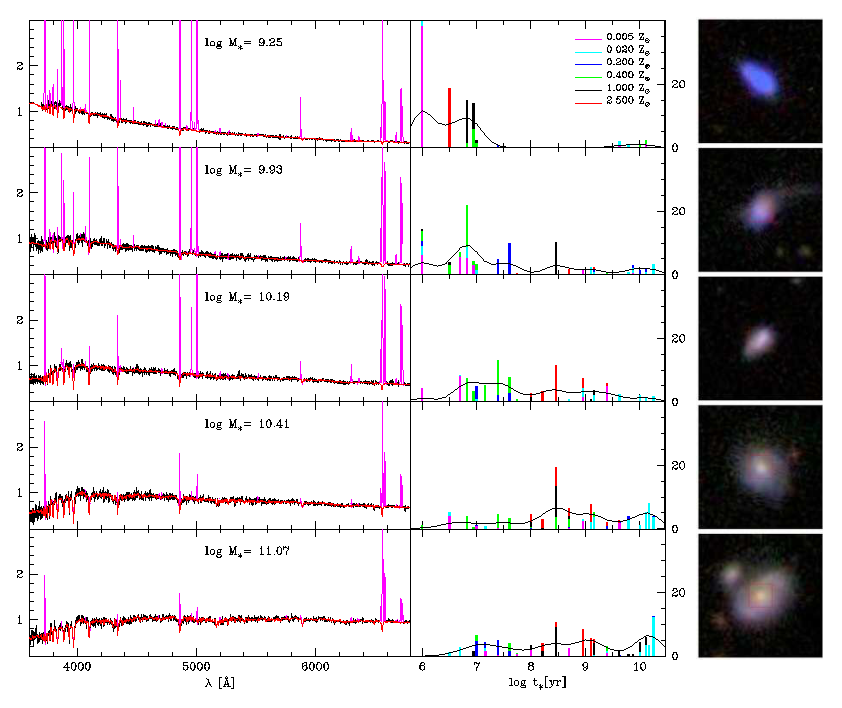
\includegraphics[width=0.7\textwidth]{figuras/starlight-fit.eps}
	\caption[Amostra de ajuste de espectro com o \starlight.]
	{Amostra de ajuste com o \starlight para o espectro de SDSS
	J1119+5130 \citep[figura 2]{CidFernandes2006}. O espectro observado é mostrado
	em preto, enquanto o modelo aparece em vermelho. Linhas de emissão (não
	modeladas) e {\em pixels} ruins são mostradas em ciano. Os espectros na parte
	inferior são a soma das SSP para as faixas de idade dadas na figura. A
	contribuição percentual no fluxo de cada grupo de idade é mostrada na legenda,
	entre parênteses.}
	\label{fig:StarlightSpectrumSample}
\end{figure}

Analisando o vetor de população das galáxias é possível obter algumas de suas
propriedades físicas. É possível também extrair as medidas das linhas de emissão
-- não modeladas no ajuste -- com bastante precisão. A técnica foi aplicada aos
espectros de galáxias do \SDSS, e o resultado da síntese gerou um catálogo de
propriedades físicas e linhas de emissão de quase um milhão de galáxias.


%***************************************************************%
%                                                               %
%                 Introdução - Este trabalho                    %
%                                                               %
%***************************************************************%

\section{Este trabalho}
\label{sec:Intro:EsteTrab}

Historicamente a região ultravioleta (UV) do espectro eletromagnético tem sido
pouco estudada na astronomia. Não por falta de interesse dos astrônomos, mas
pelo simples fato de que observações feitas de dentro da atmosfera são
impossibilitadas pela camada de ozônio. É preciso ir para o espaço. Foram
lançados diversos satélites com o intuito de estudar o céu em UV (ver seção
\ref{sec:Galex:CeuUV}). O \galex foi o primeiro telescópio espacial a fazer um
{\em survey} do céu inteiro em UV. A missão tem como objetivo estudar a evolução
da taxa de formação estelar em galáxias \citep{Martin2005}.

% FIXME: traduzir insight
Embora este e outros grandes {\em surveys} tenham um grande valor
individualmente, esta é somente a ponta do {\em iceberg}. Cruzando informações
de {\em surveys} em diversos comprimentos de onda pode-se ter novos {\em
insights}\fixme sobre a relação entre os processos físicos subjacentes. Este
trabalho utiliza dados obtidos dos {\em surveys} \SDSS e \galex, nas bandas
espectrais óptica e UV, respectivamente. Estes dois {\em surveys} foram
indexados (ver seção \ref{sec:Crossmatch:SDSSGalex}) de forma a facilitar a
identificação entre as suas detecções. A técnica desenvolvida por eles pode ser
aplicada em virtualmente qualquer outro {\em survey} astronômico.

As galáxias utilizadas na síntese do \starlight foram obtidas do catálogo do
\SDSS. Neste trabalho foi feita a identificação destas galáxias no catálogo do
\galex, obtendo-se assim as suas medidas de fotometria UV. Este conjunto de
dados formou uma amostra de galáxias com as suas propriedades físicas, cores
ópticas e cores UV. As galáxias desta amostra são classificadas utilizando o
diagrama de diagnóstico WHAN, conforme \citet{CidFernandes2011}. Este método de
classificação utiliza as linhas de emissão \Halpha e \NII para separar as
galáxias nas classes de formação estelar, núcleo ativo, ``aposentadas'' e
passivas. As cores UV das galáxias de cada classe são analisadas em busca de
correlações e tendências.

\subsection{Organização deste trabalho}

No capítulo seguinte a missão \galex é tratada em mais detalhes. As
características do {\em survey} são discutidas, e são apresentados alguns
resultados importantes. Os produtos gerados pelos {\em surveys} do \galex e o
acesso a estes dados são descritos no final do capítulo.

O terceiro capítulo introduz o uso de bancos de dados em astronomia. Em seguida
é tratado do problema genérico de identificação cruzada ({\em crossmatch}) de
objetos em catálogos de {\em surveys} astronômicos. Os bancos de dados do \SDSS
e do \starlight são apresentados, e processo de {\em crossmatch} é feito entre
os catálogos do \SDSS e do \galex. Finalmente define-se uma amostra com
magnitudes absoutas (ópticas e UV) e propriedades físícas das galáxias.

No quarto capítulo é feita a análise da amostra obtida no capítulo anterior. As
galáxias são classificadas através do diagrama WHAN e as propriedades físicas
destas galáxias (obtidas do \starlight) são analisadas de acordo com as suas
cores ópticas e UV.

No quinto e último capítulo são apresentadas as conclusões e perspectivas deste
trabalho.

As {\em queries} SQL utilizadas neste trabalho estão listadas no apêndice
\ref{apendice:Queries}.

% End of this chapter
